\documentclass[a4paper, norsk, 11pt]{scrartcl} % A4 paper and 11pt font size

\usepackage[utf8]{inputenc}
\usepackage[T1]{fontenc} % Use 8-bit encoding that has 256 glyphs
\usepackage{fourier} % Use the Adobe Utopia font for the document - comment this line to return to the LaTeX default
\usepackage{babel} % English language/hyphenation
\usepackage{amsmath,amsfonts,amsthm} % Math packages

\usepackage{lipsum} % Used for inserting dummy 'Lorem ipsum' text into the template

\usepackage{sectsty} % Allows customizing section commands
\allsectionsfont{\centering \normalfont\scshape} % Make all sections centered, the default font and small caps

\usepackage{graphicx} % Images
\usepackage{subfloat}

\usepackage{fancyhdr} % Custom headers and footers
\pagestyle{fancyplain} % Makes all pages in the document conform to the custom headers and footers
\fancyhead{} % No page header - if you want one, create it in the same way as the footers below
\fancyfoot[L]{} % Empty left footer
\fancyfoot[C]{} % Empty center footer
\fancyfoot[R]{\thepage} % Page numbering for right footer
\renewcommand{\headrulewidth}{0pt} % Remove header underlines
\renewcommand{\footrulewidth}{0pt} % Remove footer underlines
\setlength{\headheight}{13.6pt} % Customize the height of the header

\numberwithin{equation}{section} % Number equations within sections (i.e. 1.1, 1.2, 2.1, 2.2 instead of 1, 2, 3, 4)
\numberwithin{figure}{section} % Number figures within sections (i.e. 1.1, 1.2, 2.1, 2.2 instead of 1, 2, 3, 4)
\numberwithin{table}{section} % Number tables within sections (i.e. 1.1, 1.2, 2.1, 2.2 instead of 1, 2, 3, 4)

\setlength\parindent{0pt} % Removes all indentation from paragraphs - comment this line for an assignment with lots of text

%----------------------------------------------------------------------------------------
%	TITLE SECTION
%----------------------------------------------------------------------------------------

\newcommand{\horrule}[1]{\rule{\linewidth}{#1}} % Create horizontal rule command with 1 argument of height

\title{	
\normalfont \normalsize 
\textsc{TDT4117 - NTNU} \\ [25pt] % Your university, school and/or department name(s)
\horrule{0.5pt} \\[0.4cm] % Thin top horizontal rule
\huge Assignment 2 \\ % The assignment title
\horrule{2pt} \\[0.5cm] % Thick bottom horizontal rule
}

\author{Aleksander Skraastad\\
		Iver Egge} % Your name

\date{\normalsize\today} % Today's date or a custom date

\begin{document}

\maketitle % Print the title
\thispagestyle{empty} % Do not display page number on title page

%----------------------------------------------------------------------------------------

\newpage

\section{- Language model}

\textbf{1a)}

Language models are used in a variety of natural language processing.
In speech-recognition-research, probability distributions are buildt that predicts the likelyhood of a given word arising next in a sequence of tokens.\\
These probability distributions are called language models. In the case of information retrieval, a language model gives the probability that a document would generate the terms of the query, insted of that the query would generate the document.

\vspace{22pt}


%------------------------------------------------

\textbf{1b)}

\textit{q$_1$ = \{ NTNU campus \}\\}
\textit{d$_1$ = NTNU is a university in Trondheim\\}
\textit{d$_2$ = Gløshaugen is a Campus at NTNU, Øya is another campus\\}

\begin{equation*}
p(Q, d) = p(d) \Pi ((1-\lambda) p(t) + \lambda p(t | M_d))
\end{equation*}

\begin{equation*}
\lambda = {1 \over 2} = 0.5 = (1 - \lambda)
\end{equation*}

For \textit{d$_1$}

\begin{equation*}
p(q_1, d_1) = [(1 - \lambda)({2 \over 16} + {1 \over 6}) ] \times [\lambda ({2 \over 16} + {0 \over 6}) ] = ({7 \over 192}) (1 - \lambda) \lambda
\end{equation*}

For \textit{d$_2$}
\begin{equation*}
p(q_1, d_2) =[(1 - \lambda)({2 \over 16} + {1 \over 10}) ] \times [\lambda ({2 \over 16} + {2 \over 10}) ] = ({117 \over 1600}) (1 - \lambda) \lambda
\end{equation*}

Therefore
\begin{equation*}
d_2 > d_1
\end{equation*}

%----------------------------------------------------------------------------------------

\newpage

\section{- Interpolated precision}

\textbf{2a)}

Interpolated precision is used when we want to generate a more meaningful graph of recall against precision. Instead of using all the precision values we divide them into precision intervals. We can do this as the user probably wants to retrieve more documents if they are relevant.\\
Therefore, we maximize each recall-interval, and the graph becomes more ''normalized''.


\vspace{22pt}

%------------------------------------------------


\textbf{2b)}

\begin{table}[ht]
\centering
\begin{tabular}{c c c c c}
\hline
n & \# doc & Relevant & Recall & Precision \\ [0.5ex]
\hline
1 & 2 & x & $\frac{1}{4}$ & $\frac{1}{1}$  \\  
2 & 64 &  & &  \\  
3 & 72 & x & $\frac{2}{4}$ & $\frac{2}{3}$  \\  
4 & 10 &  & &  \\  
5 & 84 &  & &  \\  
6 & 15 &  & &  \\  
7 & 103 & x & $\frac{3}{4}$ & $\frac{3}{6}$  \\  
8 & 66 &  & &  \\  
9 & 37 &  & &  \\  
10 & 45 & x & $\frac{4}{4}$ & $\frac{4}{10}$  \\  
\hline
\end{tabular}
\caption{Precision and recall}
\label{prt}
\end{table}

\begin{table}[ht]
\centering
\begin{tabular}{c c c c c}
\hline
Standard recall & Precision \\ [0.5ex]
\hline
0.1 & \\
0.2 & \\
0.3 & 1.00\\
0.4 & \\
0.5 & 0.67\\
0.6 & \\
0.7 & \\
0.8 & 0.50 \\
0.9 & \\
1.0 & 0.40 \\  
\hline
\end{tabular}
\caption{Interpolated precision}
\label{ipt}
\end{table}


\begin{figure}[ht!]
\centering
\includegraphics[scale=0.6]{ip_imp3.eps}
\caption{Interpolated Precision}
\label{ipf}
\end{figure}



%----------------------------------------------------------------------------------------

\newpage

\section{- Relevance feedback}

\textbf{3a)}

Relevance feedback is to take the result from an inital query and evaluate if the result is relevant to perform a new query. The evaluation could be done by a user marking the resulting documents as relevant or not.\\

Query expansion is to process an initial query and improve the formulation of the query or match the query with other, similar queries. This could be to fix spelling errors, matching words in the query with synonyms and/or add to the result other, similar results.\\

Term reweighting is a mysterious little bastard.\\

QE and TR were separated at birth.

\vspace{22pt}

%------------------------------------------------

\textbf{3b)}

Automatic global analysis is a technique used to analyse a structured set of texts and look for word relationships (such as word context and phrase structures). Automatic local analysis instead deals with analysis of the documents retrieved by the initial query.


%----------------------------------------------------------------------------------------

\newpage

\section{- Evaluation of IR-systems}

\textbf{4a)}

Precision and Recall is a measurement of relevance of results. Precision means the fraction of the retrieved result that are relevant, and recall means the relevant fractions of the result.\\
High recall, by this definition, means that most of the relevant information is in the result, while high precision means that there are more relevant than irrelevant information in the result.\\

Formula for calculating precision
\begin{equation*}
precision = { {|\{ relevant documents \} \cap \{retrieved documents \} |} \over {| \{ retrieved documents \} |}}
\end{equation*}

Formula for calculating recall
\begin{equation*}
recall= { {|\{ relevant documents \} \cap \{retrieved documents \} |} \over {| \{ relevant documents \} |}}
\end{equation*}


\vspace{22pt}

%------------------------------------------------

\textbf{4b)}

These values are already calculated under "2 - Interpolated precision", task b (ref. table \ref{prt}).


%----------------------------------------------------------------------------------------

\end{document}